% Template LaTeX file for LAC-25 papers
%
% To generate the correct references using BibTeX, run
%     latex, bibtex, latex, latex
% modified...
% - from DAFx-00 to DAFx-02 by Florian Keiler, 2002-07-08
% - from DAFx-02 to DAFx-03 by Gianpaolo Evangelista
% - from DAFx-05 to DAFx-06 by Vincent Verfaille, 2006-02-05
% - from DAFx-06 to DAFx-07 by Vincent Verfaille, 2007-01-05
%                          and Sylvain Marchand, 2007-01-31
% - from DAFx-07 to DAFx-08 by Henri Penttinen, 2007-12-12
%                          and Jyri Pakarinen 2008-01-28
% - from DAFx-08 to DAFx-09 by Giorgio Prandi, Fabio Antonacci 2008-10-03
% - from DAFx-09 to DAFx-10 by Hannes Pomberger 2010-02-01
% - from DAFx-10 to DAFx-12 by Jez Wells 2011
% - from DAFx-12 to DAFx-14 by Sascha Disch 2013
% - from DAFx-15 to DAFx-16 by Pavel Rajmic 2015
% - from DAFx-16 to IFC-18 by Romain Michon 2018
% - from IFC-18 to LAC-19 by Romain Michon 2019
% - from LAC-19 to LAC-25 by Pierre Lecomte 2024
%
% Template with hyper-references (links) active after conversion to pdf
% (with the distiller) or if compiled with pdflatex.
%
% 20060205: added package 'hypcap' to correct hyperlinks to figures and tables
%                      use of \papertitle and \paperauthorA, etc for same title in PDF and Metadata
%
% 1) Please compile using latex or pdflatex.
% 2) If using pdflatex, you need your figures in a file format other than eps! e.g. png or jpg is working
% 3) Please use "paperftitle" and "pdfauthor" definitions below

%------------------------------------------------------------------------------------------
%  !  !  !  !  !  !  !  !  !  !  !  ! user defined variables  !  !  !  !  !  !  !  !  !  !  !  !  !  !
% Please use these commands to define title and author(s) of the paper:
\def\papertitle{The LPA Plugin: \\ A Novel Audio Plugin Architecture \\ and Development Ecosystem}
\def\paperauthorA{Joel A. Jaffe}
\def\paperauthorB{Author Two}
\def\paperauthorC{Author Three}
\def\paperauthorD{Author Four}

% Authors' affiliations have to be set below

%------------------------------------------------------------------------------------------
\documentclass[a4paper]{article}

\usepackage{style/LAC-25}
\usepackage[margin=2cm]{geometry}
\usepackage{amsmath,amssymb,amsfonts,amsthm}
\usepackage{euscript}
\usepackage[utf8]{inputenc}
\usepackage[T1]{fontenc}
\usepackage{ifpdf}
\usepackage{color}
\usepackage{listings}
\definecolor{mygrey}{rgb}{0.96,0.96,0.96}
\lstset{
  tabsize=4,
  basicstyle=\ttfamily,
  backgroundcolor=\color{mygrey},
  captionpos=b,
  breaklines=true
}

\usepackage[english]{babel}
\usepackage{caption}
\usepackage{subfig, color}

\setcounter{page}{1}
\ninept

\usepackage{times}
% Saves a lot of ouptut space in PDF... after conversion with the distiller
% Delete if you cannot get PS fonts working on your system.

% pdf-tex settings: detect automatically if run by latex or pdflatex
\newif\ifpdf
\ifx\pdfoutput\relax
\else
   \ifcase\pdfoutput
      \pdffalse
   \else
      \pdftrue
\fi

\ifpdf % compiling with pdflatex
  \usepackage[pdftex,
    pdftitle={\papertitle},
    pdfauthor={\paperauthorA, \paperauthorB, \paperauthorC, \paperauthorD},
    colorlinks=false, % links are activated as colror boxes instead of color text
    bookmarksnumbered, % use section numbers with bookmarks
    pdfstartview=XYZ % start with zoom=100% instead of full screen; especially useful if working with a big screen :-)
  ]{hyperref}
  \pdfcompresslevel=9
  \usepackage[pdftex]{graphicx}
  \usepackage[figure,table]{hypcap}
\else % compiling with latex
  \usepackage[dvips]{epsfig,graphicx}
  \usepackage[dvips,
    colorlinks=false, % no color links
    bookmarksnumbered, % use section numbers with bookmarks
    pdfstartview=XYZ % start with zoom=100% instead of full screen
  ]{hyperref}
  % hyperrefs are active in the pdf file after conversion
  \usepackage[figure,table]{hypcap}
\fi

\title{\papertitle}

%-------------SINGLE-AUTHOR HEADER STARTS (uncomment below if your paper has a single author)-----------------------
\affiliation{
\paperauthorA}
{\href{https://www.mat.ucsb.edu/}{Department of Media Arts \& Technology} \\
\href{https://www.ucsb.edu}{University of California Santa Barbara, USA} \\
{\tt \href{mailto:joel@jaffesd.com}{joel@jaffesd.com}}
}
%-----------------------------------SINGLE-AUTHOR HEADER ENDS------------------------------------------------------

%---------------TWO-AUTHOR HEADER STARTS (uncomment below if your paper has two authors)-----------------------
% \twoaffiliations{
% \paperauthorA \,\sthanks{This work was supported by the XYZ Foundation}}
% {\href{https://ccrma.stanford.edu}{CCRMA} \\ Stanford University, USA \\
% {\tt \href{mailto:lac@ccrma.stanford.edu}{lac@ccrma.stanford.edu}}
% }
% {\paperauthorB \,\sthanks{This guy is a very good fellow}}
% {\href{http://www.musikwissenschaft.uni-mainz.de/Musikinformatik/}{Johannes Gutenberg University (JGU)} \\  Mainz, Germany\\
% {\tt \href{mailto:lac@uni-mainz.de}{lac@uni-mainz.de}}
% }
%-------------------------------------TWO-AUTHOR HEADER ENDS------------------------------------------------------

%---------------THREE-AUTHOR HEADER STARTS (uncomment below if your paper has three authors)-----------------------
% \threeaffiliations{
% \paperauthorA \,\sthanks{This work was supported by the XYZ Foundation}}
% {\href{https://ccrma.stanford.edu}{CCRMA} \\ Stanford University, USA \\
% {\tt \href{mailto:lac@ccrma.stanford.edu}{lac@ccrma.stanford.edu}}
% }
% {\paperauthorB \,\sthanks{This guy is a very good fellow}}
% {\href{http://www.musikwissenschaft.uni-mainz.de/Musikinformatik/}{Johannes Gutenberg University (JGU)} \\  Mainz, Germany\\
% {\tt \href{mailto:lac@uni-mainz.de}{lac@uni-mainz.de}}
% }
% {\paperauthorC \,\sthanks{Illustrious contributor}}
% {\href{https://lmfa.ec-lyon.fr/}{LMFA} \\ Ecully, France \\
% {\tt \href{mailto:lac@ec-lyon.fr}{lac@ec-lyon.fr}}
% }
%-------------------------------------THREE-AUTHOR HEADER ENDS------------------------------------------------------

%----------------FOUR-AUTHOR HEADER STARTS (uncomment below if your paper has four authors)-----------------------
% \fouraffiliations{
% \paperauthorA \,\sthanks{This work was supported by the XYZ Foundation}}
% {\href{https://ccrma.stanford.edu}{CCRMA} \\ Stanford University, USA \\
% {\tt \href{mailto:lac@ccrma.stanford.edu}{lac@ccrma.stanford.edu}}
% }
% {\paperauthorB \,\sthanks{This guy is a very good fellow}}
% {\href{http://www.musikwissenschaft.uni-mainz.de/Musikinformatik/}{Johannes Gutenberg University (JGU)} \\  Mainz, Germany\\
% {\tt \href{mailto:lac@uni-mainz.de}{lac@uni-mainz.de}}
% }
% {\paperauthorC \,\sthanks{Illustrious contributor}}
% {\href{https://lmfa.ec-lyon.fr/}{LMFA} \\ Ecully, France \\
% {\tt \href{mailto:lac@ec-lyon.fr}{lac@ec-lyon.fr}}
% }
% {\paperauthorD \,\sthanks{Thanks to the predessors for the templates}}
% {\href{https://www.univ-st-etienne.fr}{Jean Monnet University (UJM)} \\
% Saint-Etienne, France \\
% {\tt \href{mailto:lac@univ-st-etienne.fr}{lac@univ-st-etienne.fr}}
% }
%-------------------------------------FOUR-AUTHOR HEADER ENDS------------------------------------------------------

\begin{document}
% more pdf-tex settings:
\ifpdf % used graphic file format for pdflatex
  \DeclareGraphicsExtensions{.png,.jpg,.pdf}
\else  % used graphic file format for latex
  \DeclareGraphicsExtensions{.eps}
\fi

\maketitle

\begin{abstract}
This paper introduces a novel plugin architecture, the LPA (Light-weight Plugin Architecture) plugin. 
The development of such an architecture is motivated by the expansive, duplicitous scope of existing audio plugin architectures, which are narrowly focused on deployment in DAW[] software. 
In contrast, the LPA plugin is designed to run in the widest possible variety of contexts, from bare-metal embedded systems to the Web, and everything between, while remaining language agnostic.
This is achieved by limiting the scope of the architecture to strictly perform DSP[] and provide basic parameterized control.
\end{abstract}

\section{Introduction}
\label{sec:intro}

The term "audio plugin" in 2025[], for those who have some association with it, mostly denotes a binary executable designed to run inside DAW software. 
More broadly, the term audio plugin can describe any audio-focused program designed to operate inside a host application, which does not necessarily have to be audio specific. 
Examples include audio plugins for software 3D and animation software such as Blender[], game engines such as Unity[] and Unreal[], and even the browser[]. 
Given that these plugins all operate on the same core data structures, it is both possible and desirable to maintain audio DSP codebases that can deploy to multiple of these plugin formats, as well as standalone applications, from the same source code.

The concept of "write once, run anywhere" (WORA) transcends the audio DSP realm, of course. 
Notably, it was a slogan for the Java[] programming language when it was introduced in 1995, and the explosion of Web based technologies can be seen as a direct descendent. 
In the audio DSP world, different approaches to WORA can be broadly categorized as being one of two types.

has mainly been seen in the case of domain-specific languages and runtimes.


One approach is 

tool oriented towards this is FAUST[], a domain-specific programming language for real-time DSP. FAUST affords the programmer the ability to define audio processing without having to manually manage memory, and to target multiple different deployments from the same code. The downside of the bargain is that the programmer must learn Faust.

Note: Figure 17 of "FAUST Domain Specific Audio DSP Language Compiled to WebAssembly" shows the performance of FAUST->C->emcc->wasm roughly equal to FAUST->wasm.

A node-oriented option is Gen\~~. Gen\~~ affords the ability to create efficient, low-level[] audio processing without having to write code at all, yet also exposes a textual code interface for advanced users. Like FAUST, Gen also deploys to many targets, by generating code.

A downside of these DSL approaches is that they constrain the programmer to writing traditional DSP code, being poor choices for implementing modern techniques, such as neural audio inference engines[].

A language-agnostic tool would be great.

The definition of this is found in an audio plugin standard as defined in DAWS: a piece of executable binary[] that can have come from any, including multiple, programming language(s).

\section{Related Work}
\label{ssec:Related Work}

All figures should be centered on the column (or page, if the figure spans both
columns). Figure captions (in italic) should follow each figure and have the
format given in Figure~\ref{fft_plot}. Vectorial figures are preferred (e.g.,
Postscript, PDF, etc.). Also, in order to provide a better readability, figure
text font size should be at least identical to footnote font size. If bitmap
figures are used, please make sure that the resolution is enough for print
quality. Figure~\ref{ftt_plot2} illustrates an example of a figure spanning two
columns.

\begin{figure}[ht]
\centerline{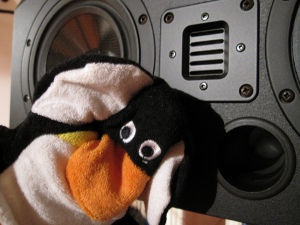
\includegraphics[scale=0.5]{figures/ping}}
\caption{\label{fft_plot}{\it Ping.}}
\end{figure}

\begin{figure*}[ht]
\center
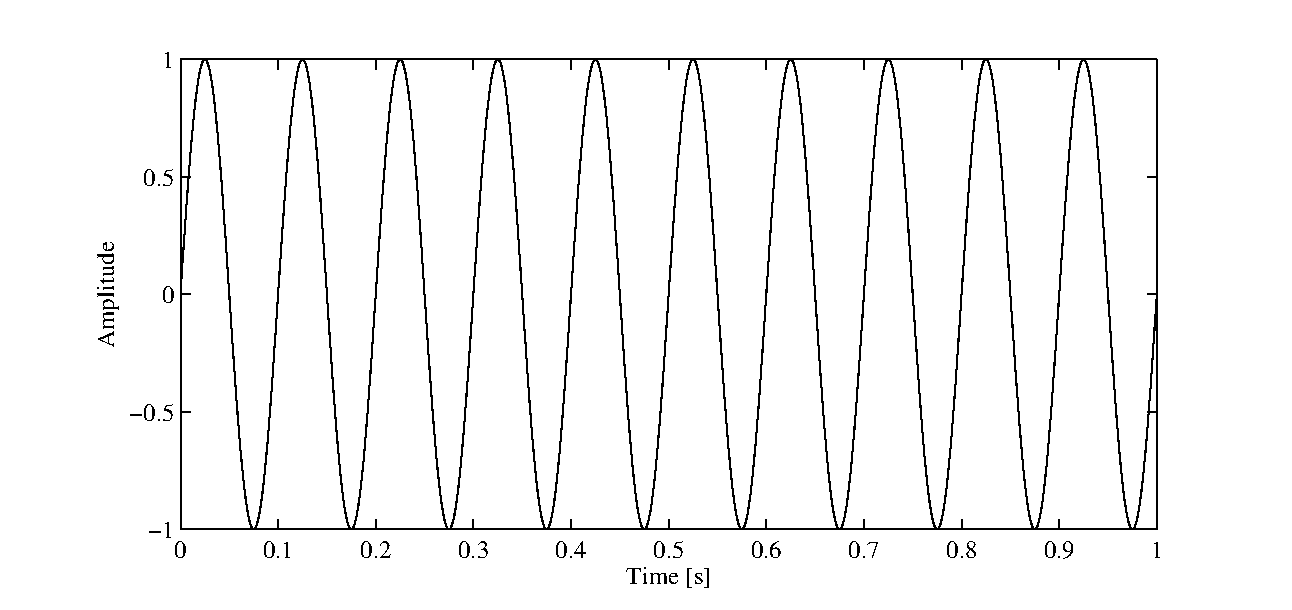
\includegraphics[width=5in]{figures/TwoColumnSine2/TwoColumnSine2}
\caption{\label{ftt_plot2}{\it A figure spanning two columns, as mentioned in
Sec. \ref{ssec:figures}.}}
\end{figure*}

\subsection{Domain-Specific Programming for Audio DSP (FAUST and Gen\~~)}
\subsection{Gen~}
\subsection{Cool Third Thing}
\section{The LPA Standard}
\section{Developer Tooling}
\section{Evaluation}
\section{Conclusion}
\section{Acknowledgments}

As for figures, all tables should be centered on the column (or page, if the
table spans both columns). Table captions should be in italic, precede each
table and have the format given in Table~\ref{tab:example}.

\begin{table}[ht]
  \caption{\itshape Basic trigonometric values.}
	\centering
	\begin{tabular}{|c|c|}
		\hline
		$\mathrm{angle}\,(\theta, \mathrm{rad})$ & $\sin \theta$ \\\hline
		$\frac{\pi}{2}$ & $1$ \\
		$\pi$ & $0$ \\
		$\frac{3\pi}{2}$ & $-1$ \\
		$2\pi$ & $0$ \\\hline
	\end{tabular}
	%
	\label{tab:example}
\end{table}

\begin{table*}[ht]
  \caption{{\it Basic trigonometric values, spanning two columns.}}
	\centering
  \begin{tabular}{|c|c|c|c|c|c|c|}\hline
    $\mathrm{angle}\, (\theta, \mathrm{rad})$ & $\sin \theta$ & $\cos \theta $ & $(\sin \theta)/2 $ & $(\cos \theta) /2 $ & $(\sin \theta)/3 $ & $(\cos \theta)/3$    \\\hline
    $\frac{\pi}{2}$ & $1$ & $0$ & $1/2$ & $0$ & $1/3$ & $0$ \\
    $\pi$ & $0$ & $-1$ & $0$ & $-1/2$ & $0$ & $-1/3$\\
    $\frac{3\pi}{2}$ & $-1$ & $0$ & $-1/2$ & $0$ & $-1/3$ & $0$ \\
    $2\pi$ & $0$ & $1$ & $0$ & $1/2$ & $0$ & $1/3$ \\\hline
 \end{tabular}
	%
  \label{tab:example2}
\end{table*}

\subsection{Equations}

Equations should be placed on separate lines and numbered:

\begin{equation}
	y(n)=b_0x(n)-a_1y(n-1)
	\label{eq1}
	\end{equation}
	where equation (\ref{eq1}) is a one pole filter with frequency response:
	\begin{equation}
	H(e^{j \omega T}) = \frac{b_0}{1+a_1e^{-j \omega T}}
	\label{eq2}
\end{equation}

\subsection{Code}

Code can be listed in a block:

\begin{lstlisting}
  int foo = 0;
\end{lstlisting}
\noindent
or directly in-lined in the body of the text: \lstinline{int foo = 1;}.

\subsection{Page Numbers}

Page numbers will be added to the document in the post-processing stage, so
{\em please leave the numbering as is} (no numbers).


\subsection{References}

The references will be numbered in order of appearance \cite{Sal89},
\cite{Spa72}, \cite{MosWal64} and \cite{Kay86}. Please avoid listing
references that do not appear in the text.

\subsubsection{Reference Format}

The reference format is the standard IEEE one. We recommend to use BibTeX to
create the reference list.

\section{Conclusions}

This template can be found on the conference website. For changing the number
of author affiliations (1 to 4), uncomment the corresponding regions in the
template \texttt{tex} file. Please, submit full-length papers (4 to 8 pages
for full papers and 2 to 4 pages for poster papers) and keep the paper size to
letter (don't change to A4). Submission is fully electronic and automated 
through the Conference Web Submission System. DO NOT send us papers directly by 
e-mail.

\section{Acknowledgments}

Many thanks to the great number of anonymous reviewers!

%\newpage
\nocite{*}
\bibliographystyle{style/IEEEbib}
\bibliography{style/LAC-25} % requires file lac-25.bib

\section{Appendix: Margin Check}

This section shows the column margins for the text.

Lorem ipsum dolor sit amet, consectetur adipisici elit, sed eiusmod tempor
incidunt ut labore et dolore magna aliqua. Ut enim ad minim veniam, quis
nostrud exercitation ullamco laboris nisi ut aliquid ex ea commodi consequat.
Quis aute iure reprehenderit in voluptate velit esse cillum dolore eu fugiat
nulla pariatur. Excepteur sint obcaecat cupiditat non proident, sunt in culpa
qui officia deserunt mollit anim id est laborum.

Duis autem vel eum iriure dolor in hendrerit in vulputate velit esse molestie
consequat, vel illum dolore eu feugiat nulla facilisis at vero eros et accumsan
et iusto odio dignissim qui blandit praesent luptatum zzril delenit augue duis
dolore te feugait nulla facilisi. Lorem ipsum dolor sit amet, consectetuer
adipiscing elit, sed diam nonummy nibh euismod tincidunt ut laoreet dolore
magna aliquam erat volutpat.

Ut wisi enim ad minim veniam, quis nostrud exerci tation ullamcorper suscipit
lobortis nisl ut aliquip ex ea commodo consequat. Duis autem vel eum iriure
dolor in hendrerit in vulputate velit esse molestie consequat, vel illum dolore
eu feugiat nulla facilisis at vero eros et accumsan et iusto odio dignissim qui
blandit praesent luptatum zzril delenit augue duis dolore te feugait nulla
facilisi.

Nam liber tempor cum soluta nobis eleifend option congue nihil imperdiet doming
id quod mazim placerat facer possim assum. Lorem ipsum dolor sit amet,
consectetuer adipiscing elit, sed diam nonummy nibh euismod tincidunt ut
laoreet dolore magna aliquam erat volutpat. Ut wisi enim ad minim veniam, quis
nostrud exerci tation ullamcorper suscipit lobortis nisl ut aliquip ex ea
commodo consequat.

Duis autem vel eum iriure dolor in hendrerit in vulputate velit esse molestie
consequat, vel illum dolore eu feugiat nulla facilisis.

At vero eos et accusam et justo duo dolores et ea rebum. Stet clita kasd
gubergren, no sea takimata sanctus est Lorem ipsum dolor sit amet. Lorem ipsum
dolor sit amet, consetetur sadipscing elitr, sed diam nonumy eirmod tempor
invidunt ut labore et dolore magna aliquyam erat, sed diam voluptua. At vero
eos et accusam et justo duo dolores et ea rebum. Stet clita kasd gubergren, no
sea takimata sanctus est Lorem ipsum dolor sit amet. Lorem ipsum dolor sit
amet, consetetur sadipscing elitr, At accusam aliquyam diam diam dolore dolores
duo eirmod eos erat, et nonumy sed tempor et et invidunt justo labore Stet
clita ea et gubergren, kasd magna no rebum. sanctus sea sed takimata ut vero
voluptua. est Lorem ipsum dolor sit amet. Lorem ipsum dolor sit amet,
consetetur sadipscing elitr, sed diam nonumy eirmod tempor invidunt ut labore
et dolore magna aliquyam erat.

Consetetur sadipscing elitr, sed diam nonumy eirmod tempor invidunt ut labore
et dolore magna aliquyam erat, sed diam voluptua. At vero eos et accusam et
justo duo dolores et ea rebum. Stet clita kasd gubergren, no sea takimata
sanctus est Lorem ipsum dolor sit amet. Lorem ipsum dolor sit amet, consetetur
sadipscing elitr, sed diam nonumy eirmod tempor invidunt ut labore et dolore
magna aliquyam erat, sed diam voluptua. At vero eos et accusam et justo duo
dolores et ea rebum. Stet clita kasd gubergren, no sea takimata sanctus est
Lorem ipsum dolor sit amet. Lorem ipsum dolor sit amet, consetetur sadipscing
elitr, sed diam nonumy eirmod tempor invidunt ut labore et dolore magna aliquyam
erat, sed diam voluptua. At vero eos et accusam et justo duo dolores et ea
rebum. Stet clita kasd gubergren, no sea takimata sanctus est Lorem ipsum dolor
sit amet.

Lorem ipsum dolor sit amet, consectetur adipisici elit, sed eiusmod tempor
incidunt ut labore et dolore magna aliqua. Ut enim ad minim veniam, quis
nostrud exercitation ullamco laboris nisi ut aliquid ex ea commodi consequat.
Quis aute iure reprehenderit in voluptate velit esse cillum dolore eu fugiat
nulla pariatur. Excepteur sint obcaecat cupiditat non proident, sunt in culpa
qui officia deserunt mollit anim id est laborum.


Duis autem vel eum iriure dolor in hendrerit in vulputate velit esse molestie
consequat, vel illum dolore eu feugiat nulla facilisis at vero eros et accumsan
et iusto odio dignissim qui blandit praesent luptatum zzril delenit augue duis
dolore te feugait nulla facilisi. Lorem ipsum dolor sit amet, consectetuer
adipiscing elit, sed diam nonummy nibh euismod tincidunt ut laoreet dolore
magna aliquam erat volutpat.

Ut wisi enim ad minim veniam, quis nostrud exerci tation ullamcorper suscipit
lobortis nisl ut aliquip ex ea commodo consequat. Duis autem vel eum iriure
dolor in hendrerit in vulputate velit esse molestie consequat, vel illum dolore
eu feugiat nulla facilisis at vero eros et accumsan et iusto odio dignissim qui
blandit praesent luptatum zzril delenit augue duis dolore te feugait nulla
facilisi.

Nam liber tempor cum soluta nobis eleifend option congue nihil imperdiet doming
id quod mazim placerat facer possim assum. Lorem ipsum dolor sit amet,
consectetuer adipiscing elit, sed diam nonummy nibh euismod tincidunt ut
laoreet dolore magna aliquam erat volutpat. Ut wisi enim ad minim veniam, quis
nostrud exerci tation ullamcorper suscipit lobortis nisl ut aliquip ex ea
commodo consequat.

Duis autem vel eum iriure dolor in hendrerit in vulputate velit esse molestie
consequat, vel illum dolore eu feugiat nulla facilisis.

At vero eos et accusam et justo duo dolores et ea rebum. Stet clita kasd
gubergren, no sea takimata sanctus est Lorem ipsum dolor sit amet. Lorem ipsum
dolor sit amet, consetetur sadipscing elitr, sed diam nonumy eirmod tempor
invidunt ut labore et dolore magna aliquyam erat, sed diam voluptua. At vero
eos et accusam et justo duo dolores et ea rebum. Stet clita kasd gubergren, no
sea takimata sanctus est Lorem ipsum dolor sit amet. Lorem ipsum dolor sit amet,
consetetur sadipscing elitr, At accusam aliquyam diam diam dolore dolores duo
eirmod eos erat, et nonumy sed tempor et et invidunt justo labore Stet clita ea
et gubergren, kasd magna no rebum. sanctus sea sed takimata ut vero voluptua.
est Lorem ipsum dolor sit amet. Lorem ipsum dolor sit amet, consetetur
sadipscing elitr, sed diam nonumy eirmod tempor invidunt ut labore et dolore
magna aliquyam erat.

Consetetur sadipscing elitr, sed diam nonumy eirmod tempor invidunt ut labore
et dolore magna aliquyam erat, sed diam voluptua. At vero eos et accusam et
justo duo dolores et ea rebum. Stet clita kasd gubergren, no sea takimata
sanctus est Lorem ipsum dolor sit amet. Lorem ipsum dolor sit amet, consetetur
sadipscing elitr, sed diam nonumy eirmod tempor invidunt ut labore et dolore
magna aliquyam erat, sed diam voluptua. At vero eos et accusam et justo duo
dolores et ea rebum. Stet clita kasd gubergren, no sea takimata sanctus est
Lorem ipsum dolor sit amet.

\end{document}
